\documentclass{article}

% Packages
\usepackage[utf8]{inputenc}

\usepackage{amsmath, bm}
\usepackage{graphicx}
\usepackage{amssymb}
\usepackage{float}
\usepackage{caption}
\usepackage{subcaption}
\usepackage{geometry}
\usepackage{multirow}
\usepackage{hyperref}

\newgeometry{vmargin={1in}, hmargin={1in}}


\title{3A1 Transition to Turbulence Lab Report}
\author{[Louis Pender]}
\date{February 29, 2024}

\begin{document}

\maketitle

\section{Objectives}

\begin{itemize}
    \item To observe with the aid of a hot-wire anemometer and a stethoscope the transition
    from a laminar to a turbulent boundary layer on a flat plate:
    \begin{itemize}
        \item when smooth
        \item behind an isolated roughness element on the centre-line of the plate
        \item behind a two-dimensional roughness trip
    \end{itemize}
    
    \item To obtain the transition Reynolds numbers for the above conditions.
    \item To measure the angle of the turbulent wedge that is formed downstream of the roughness element.
    \item To measure the mean and turbulent profiles of the boundary layer when it is fully turbulent.
    \item To use the mean flow velocity profile to estimate the skin friction co-efficient. % On Clauser Plot
\end{itemize}


\section{Theory}
% Describe the experimental setup, equipment used, and the steps followed during the experiment.

\subsection{Hot wire anemometry}

The hot wire anemometer is a device used to measure the velocity of a fluid.
The wires resistance changes with temperature and the convective heat loss is related to the velocity of the fluid.
This is measured by a Wheatstone bridge circuit which is balanced at a constant temperatue.
The heat loss of the wire can be modelled by King's Law
\begin{equation}
    E^2 = A + B U^{\frac{1}{2}}
\end{equation}
Considering a turbulent flow the velocity profile can be modelled as $\bar{U} + U'$ and similarly, a voltage $\bar{E} + E'$ which represents the sum of a mean value and a fluctuating component.
Additionally the following relation holds:
\begin{equation}
    \frac{E'}{U'} = \frac{d\bar{E}}{d\bar{U}}
\end{equation}
This can be substituted into the King's Law to give
\begin{equation}
    \frac{U'}{E'} = \frac{4\bar{E}\bar{U}^{\frac{1}{2}}}{B} = \frac{4\bar{E}(\bar{E}^2 - A)}{B^2}
    \label{eq:small_kings}
\end{equation}

The parameter that governs the transition to turbulent flow is the Reynolds number based on the distance $x$ from the leading edge of the plate.
\begin{equation}
    Re_x = \frac{\rho \bar{U}x}{\mu}
\end{equation}

A turbulent boundary layer profile can be approximated by the log law seen below \cite{notes}:
\begin{equation}
    \frac{u}{u_*} = \frac{1}{\kappa} \ln \left( \frac{y u_*}{\nu} \right) + B
\end{equation}
Where $u_*$ is the friction velocity, $y$ is the distance from the wall, and $\nu$ is the kinematic viscosity of the fluid.
The values of $\kappa$ and $B$ are constants which are taken as 0.41 and 5.0 respectively.
This profile was derived for an overlapping region of the boundary layer, where both turbulent and viscous shear stresses are significant.
However, in this case it can be used to approximate the entire boundary layer profile as the inner law region is small and the effect of the outer law is small over the pressure gradient.

The friction velocity is defined as follows from the skin friction coefficient $C_f$:
\begin{equation}
    U_* = \left( \frac{\tau}{\rho} \right)^{\frac{1}{2}} = \left[ \frac{1}{2}C_f \bar{ U}_1^2 \right]^{\frac{1}{2}}
    \label{eq:friction_velocity}
\end{equation}

The size of turbulent spots can be estimated by measuring the time of the turbulent noise regions on the oscilloscope, and multiplying by the local velocity.
Similarly the size of a typical eddy can be estimated by finding the average time between turbulent peaks and multiplying by only the local fluctuating velocity.
This is because the eddies are thought to move at the local velocity of the fluid. % Is this true?

The figure below shows stages of transition to turbulence in a boundary layer flow where Tollmien-Schlichting waves are formed and grow, leading to the formation of turbulent spots and eddies.
\begin{figure}[H]
    \centering
    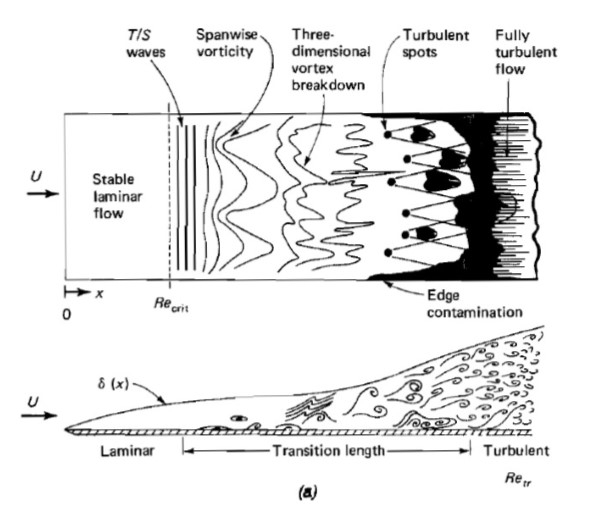
\includegraphics[width=0.6\textwidth]{transition_stages.jpg}
    \caption{Transition stages of a boundary layer flow \cite{textbook}}
    \label{fig:transition_stages}
\end{figure}
% The actual transition from laminar to turbulent boundary layer flow may occur over a region of the plate, not at a single point.

%%%%%%%%%%%%%%%%%%%%

\section{Results}
% Present the data obtained from the experiment, including tables, graphs, and figures.

The density of air $\rho = 1.225kgm^{-3}$ for the standard atmosphere with $15^\circ C$ and 760 mmHg
At these standard conditions the viscosity of air is $1.48 \times 10^{-5} Ns/m^2$.

\begin{figure}[H]
    \centering
    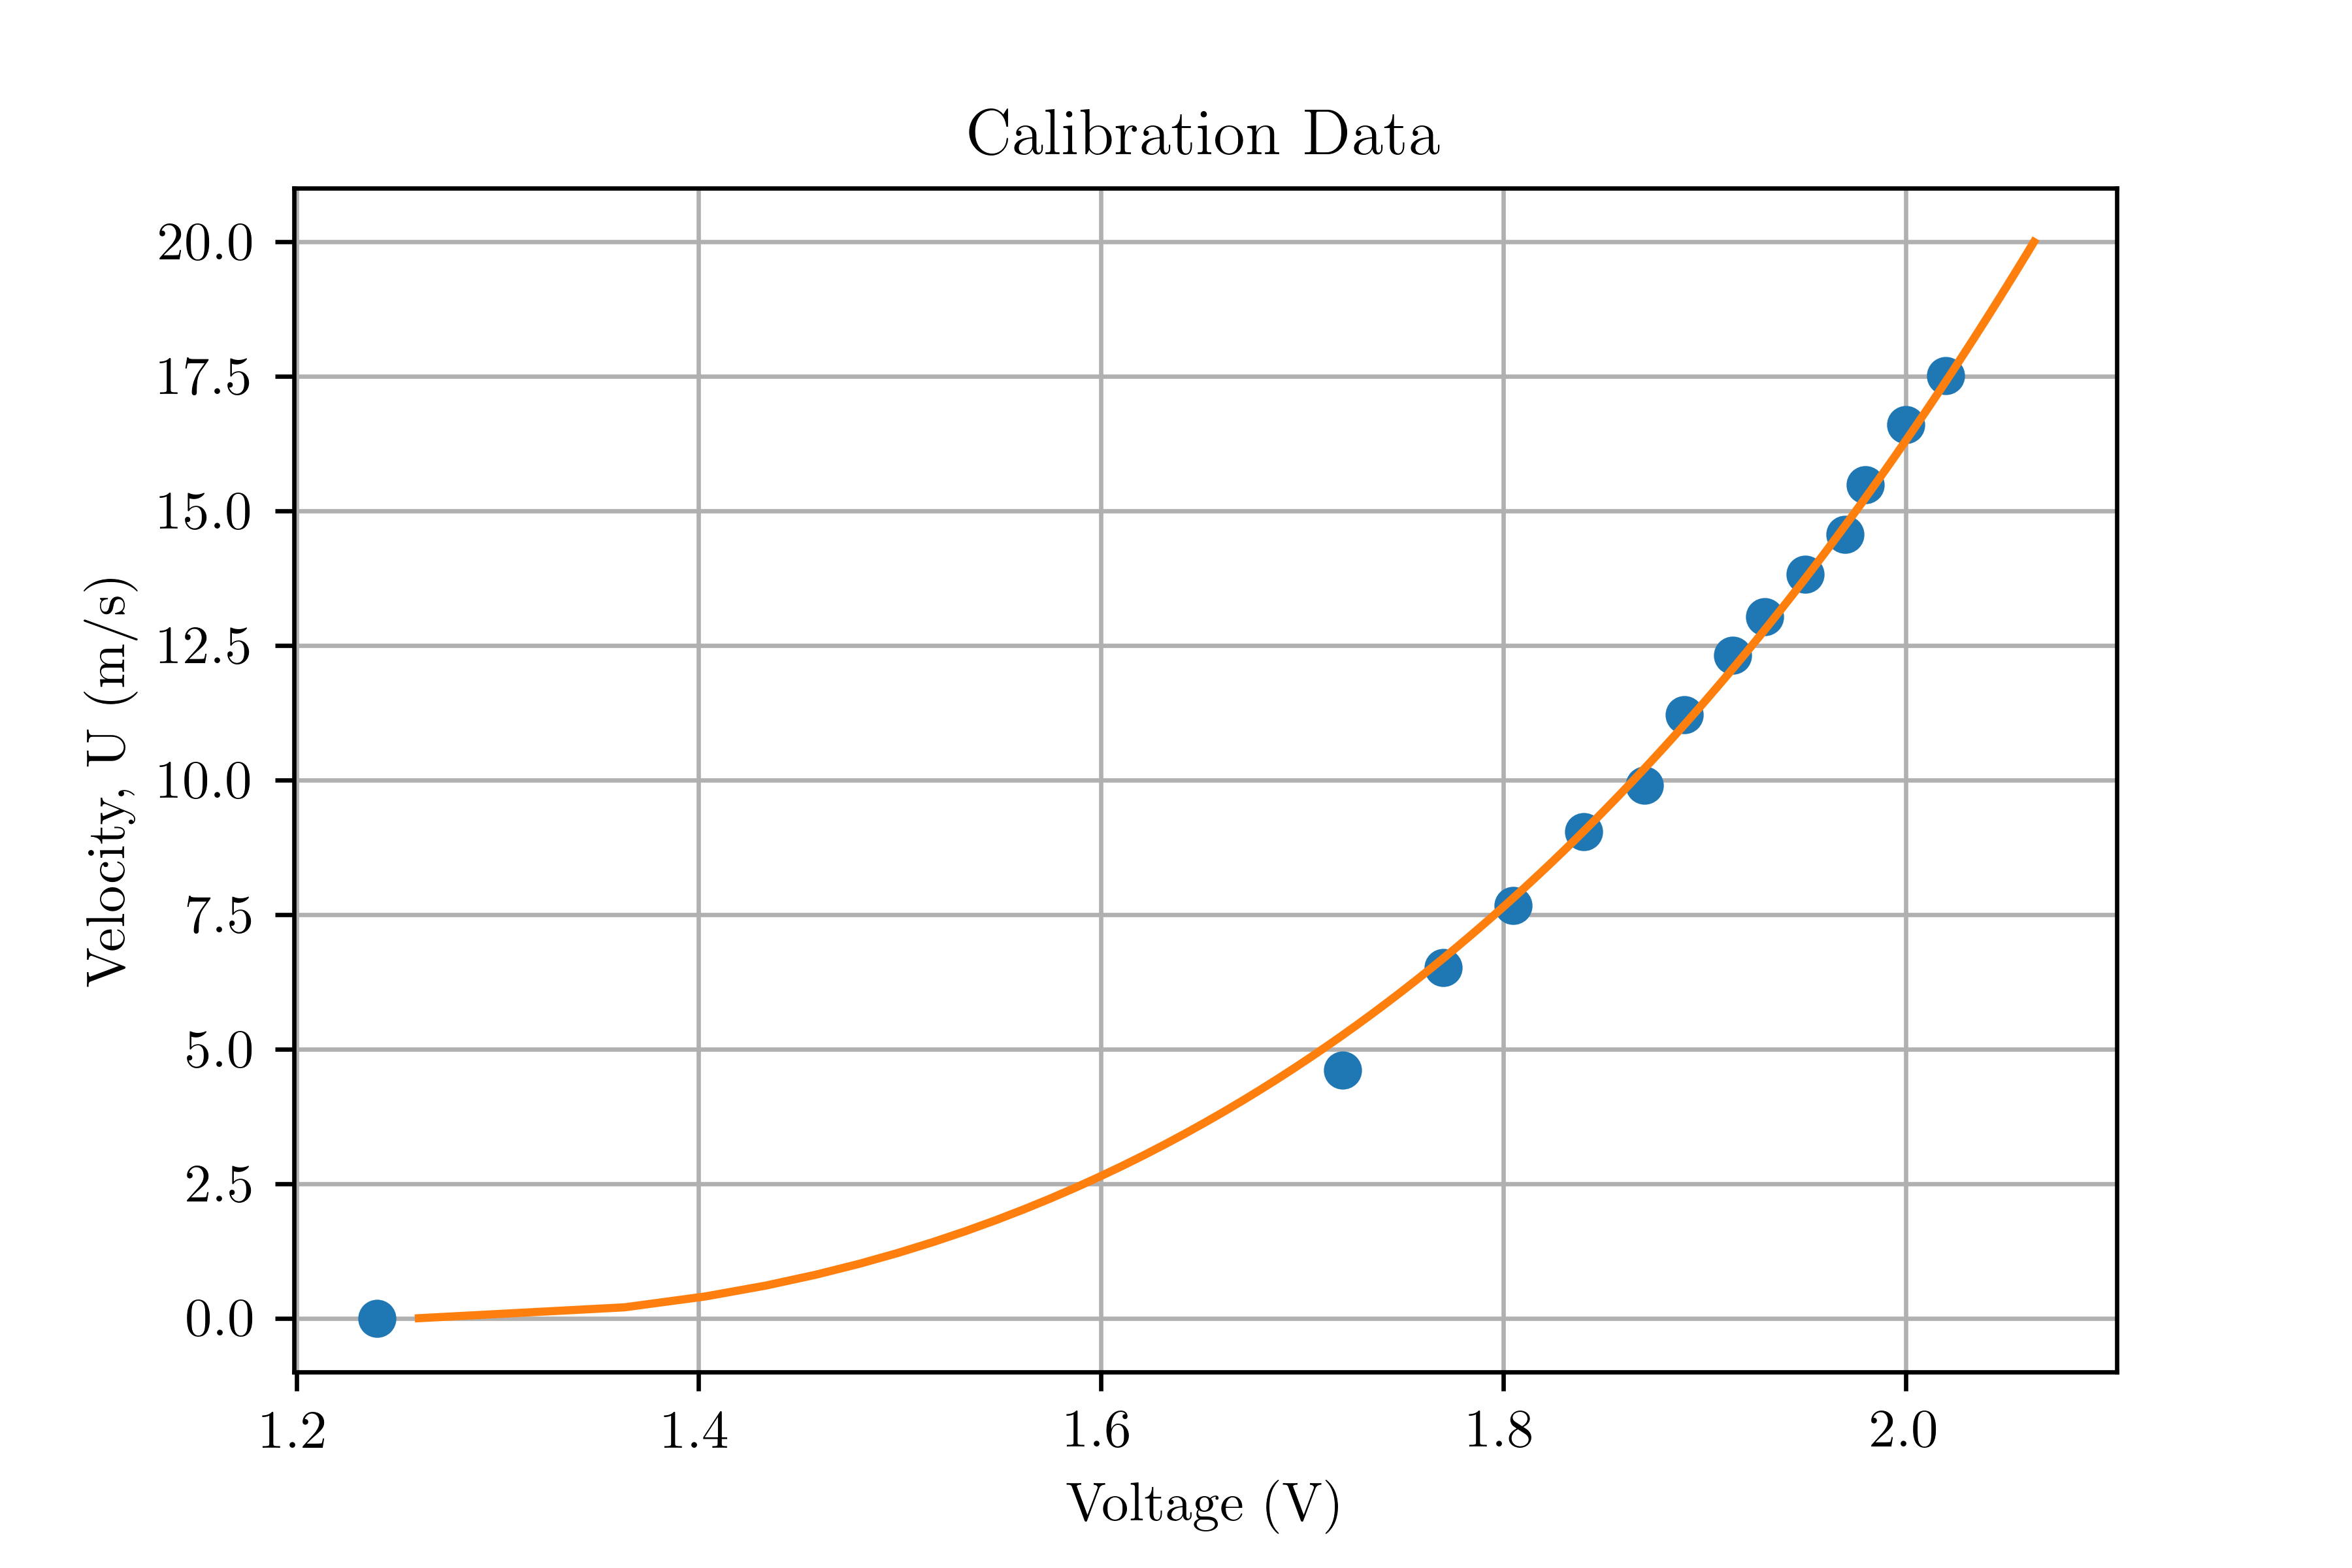
\includegraphics[width=0.8\textwidth]{calibration.png}
    \caption{Calibration curve for the hot wire anemometer}
    \label{fig:calibration}
\end{figure}


\begin{table}[H]
    \centering
    \begin{tabular}{cccccccc}
        \hline
        \multirow{2}{*}{Setup} &  Dial &  $\Delta p$ &  $U_{\infty}$ &  $Re_x$ & $\bar{U}$ & $U'$ & \multirow{2}{*}{Comment} \\
        &(-)&(mBar)&(m/s)&(-)&(m/s)&(m/s)&  \\
        \hline
        \hline
        \multirow{4}{*}{Flat Plate} & 300 & 0.11 & 4.238 & $4.00 \times 10^5$ & 1.415 & 0.08192 & Laminar \\
        & 650 & 1.04 & 13.031 & $1.23 \times 10^6$ & 7.902 & 0.77506 & Transitioning \\
        & 820 & 1.59 & 16.112 & $1.52 \times 10^6$ & 11.066 & 0.005055\footnote[1]{}  & Transitioning \\
        & 1000 & 2.1 & 18.516 & $1.75 \times 10^6$ & 13.253 & 0.5953 & Turbulent \\
        \hline
        \hline
        \multirow{3}{*}{Protrusion} & 300 & 0.11 & 4.238 & $4.00 \times 10^5$ & 1.610 & 0.2600 & Laminar \\
        & 370 & 0.34 & 7.4505 & $7.03 \times 10^6$ & 3.519 & 0.6765 & Transitioning \\
        & 430 & 0.47 & 8.7598 & $8.27 \times 10^6$ & 5.178 & 0.6769 & Turbulent \\
        \hline
        \hline
        \multirow{1}{*}{Trip Wire} & 200 & 0.04 & 2.556 & $2.41 \times 10^5$ & 1.159 & 0.5855 & Turbulent \\
        \hline
    \end{tabular}
    \caption{Observations and Reynolds numbers for various arrangements of the tunnel.}
    \label{tab:observations}
\end{table}

\begin{table}[H]
    \centering
    \begin{tabular}{ccccccc}
        \hline
        \multirow{2}{*}{Setup} & Dial & $Re_x$ & $\Delta T_{\text{spot}}$ & $\Delta T_{\text{peak}}$ & Spot Size & Eddy Size \\
        & (-) & (-) & (ms) & (ms) & (mm) & (mm) \\
        \hline
        \hline
        \multirow{3}{*}{Flat Plate} & 650 & $1.23 \times 10^6$ & 25 & 6.25 & 35.363 & 4.8441 \\
        & 820 & $1.52 \times 10^6$ & 200 & 8.33 & 1580.4 & 0.04213\footnotemark \\
        & 1000 & $1.75 \times 10^6$ & - & 5.00 & - & 2.9766 \\
        \hline
        \hline
        \multirow{2}{*}{Protrusion} & 370 & $7.03 \times 10^6$ & 42.5 & 7.08 & 28.753 & 4.792        \\
        & 430 & $8.27 \times 10^6$ & - & 7.14 & - & 4.835 \\
        \hline
        \hline
        \multirow{1}{*}{Trip Wire} & 200 & $2.41 \times 10^5$ & - & 16.7 & - & 9.758 \\
        \hline
    \end{tabular}
    \caption{Spot and Eddy sizes for turbulent and transitioning boundary layers.}
    \label{tab:spot_sizes}
\end{table}

\footnotetext{ The value of $E'$ recorded for this calculation is believed to be an error}

\begin{figure}[H]
    \centering 
    \begin{subfigure}{0.8\textwidth}
        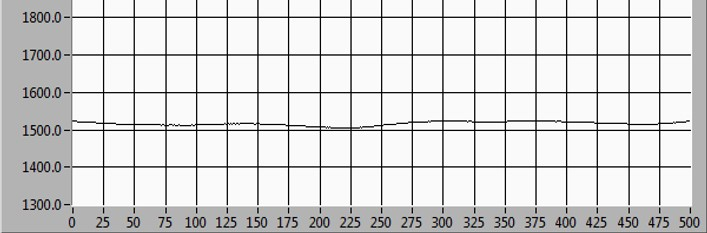
\includegraphics[width=\textwidth]{1_laminar.jpg}
        \caption{Laminar boundary layer at 300 dial}
        \label{fig:oscilloscope_laminar}
    \end{subfigure}
    \begin{subfigure}{0.8\textwidth}
        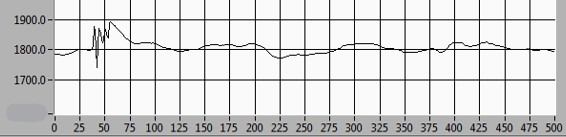
\includegraphics[width=\textwidth]{2_transition.jpg}
        \caption{Transitioning boundary layer at 650 dial}
        \label{fig:oscilloscope_mostly_laminar}
    \end{subfigure}
    \begin{subfigure}{0.8\textwidth}
        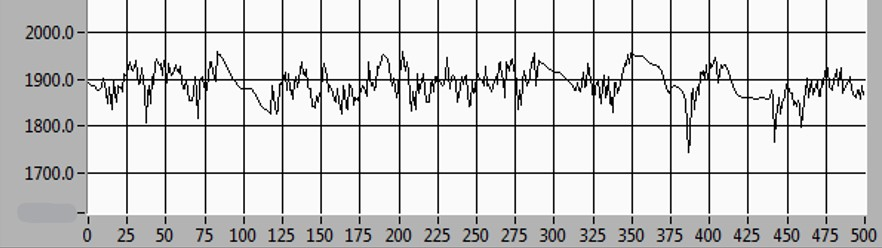
\includegraphics[width=\textwidth]{3_transition.jpg}
        \caption{Transitioning boundary layer at 820 dial}
        \label{fig:oscilloscope_mostly_turbulent}
    \end{subfigure}
    \begin{subfigure}{0.8\textwidth}
        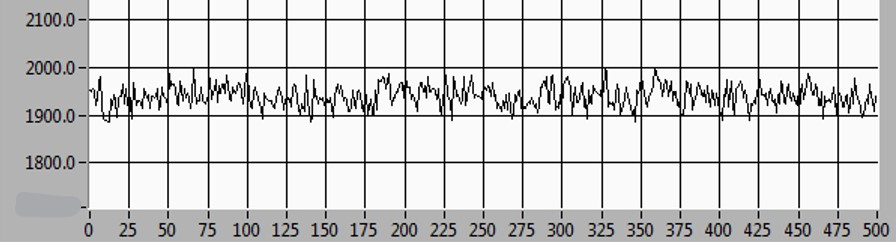
\includegraphics[width=\textwidth]{4_turbulent.jpg}
        \caption{Turbulent boundary layer at 1000 dial}
        \label{fig:oscilloscope_turbulent}
    \end{subfigure}
    \caption{Aenometer oscilloscope readings for various tunnel speeds for the flat plate at a distance of 0.2mm}
    \label{fig:oscilloscope}
\end{figure}

%% microphone readings

\begin{figure}[H]
    \centering
    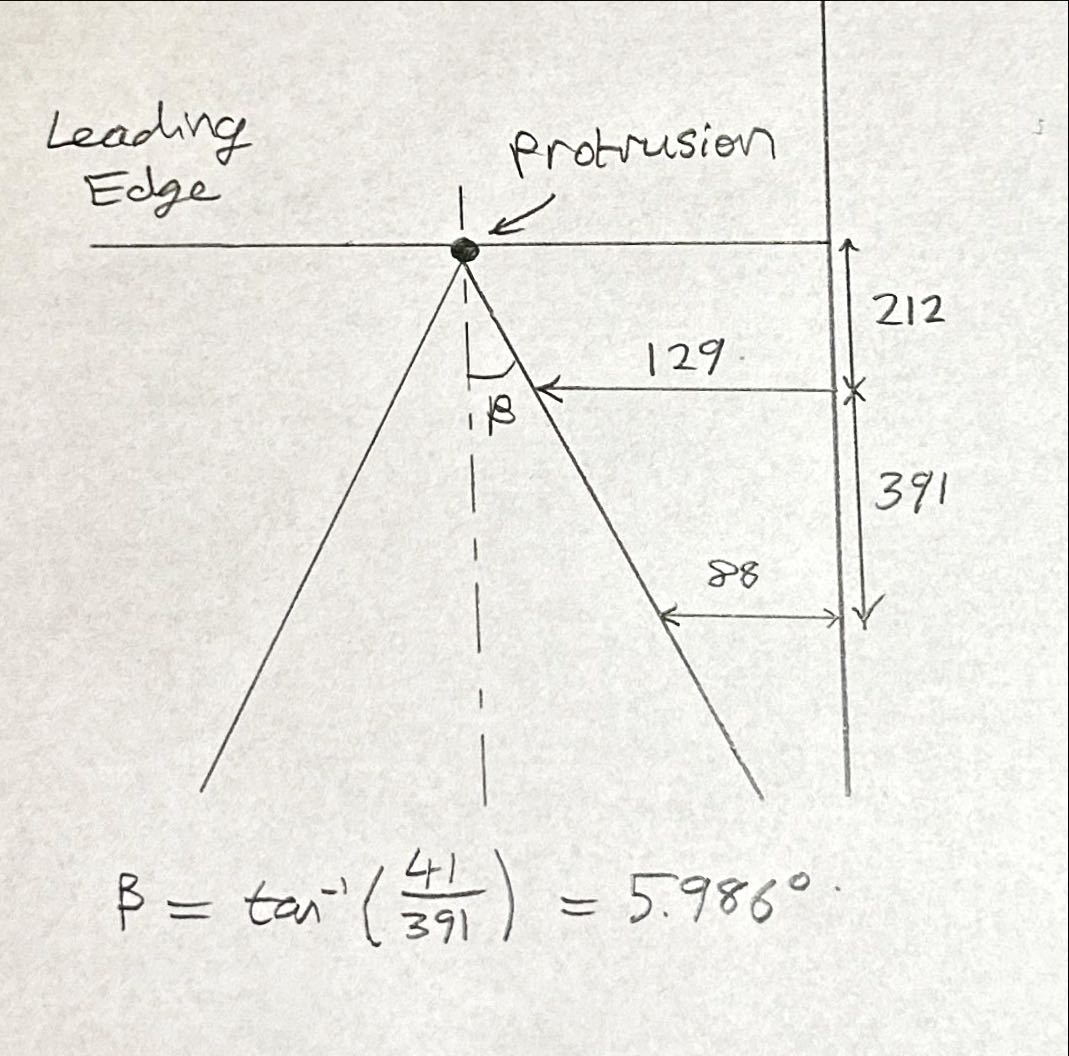
\includegraphics[width=0.5\textwidth]{turbulent_wedge.jpg}
    \caption{Angle of turbulent wedge formed downstream of the protrusion. The angle was found to be $\beta \approx 6^\circ$ at a dial setting of 400.}
    \label{fig:turbulent_wedge}
\end{figure}

% 1. Express your results in terms of the Reynolds number.

\begin{figure}[H]
    \centering
    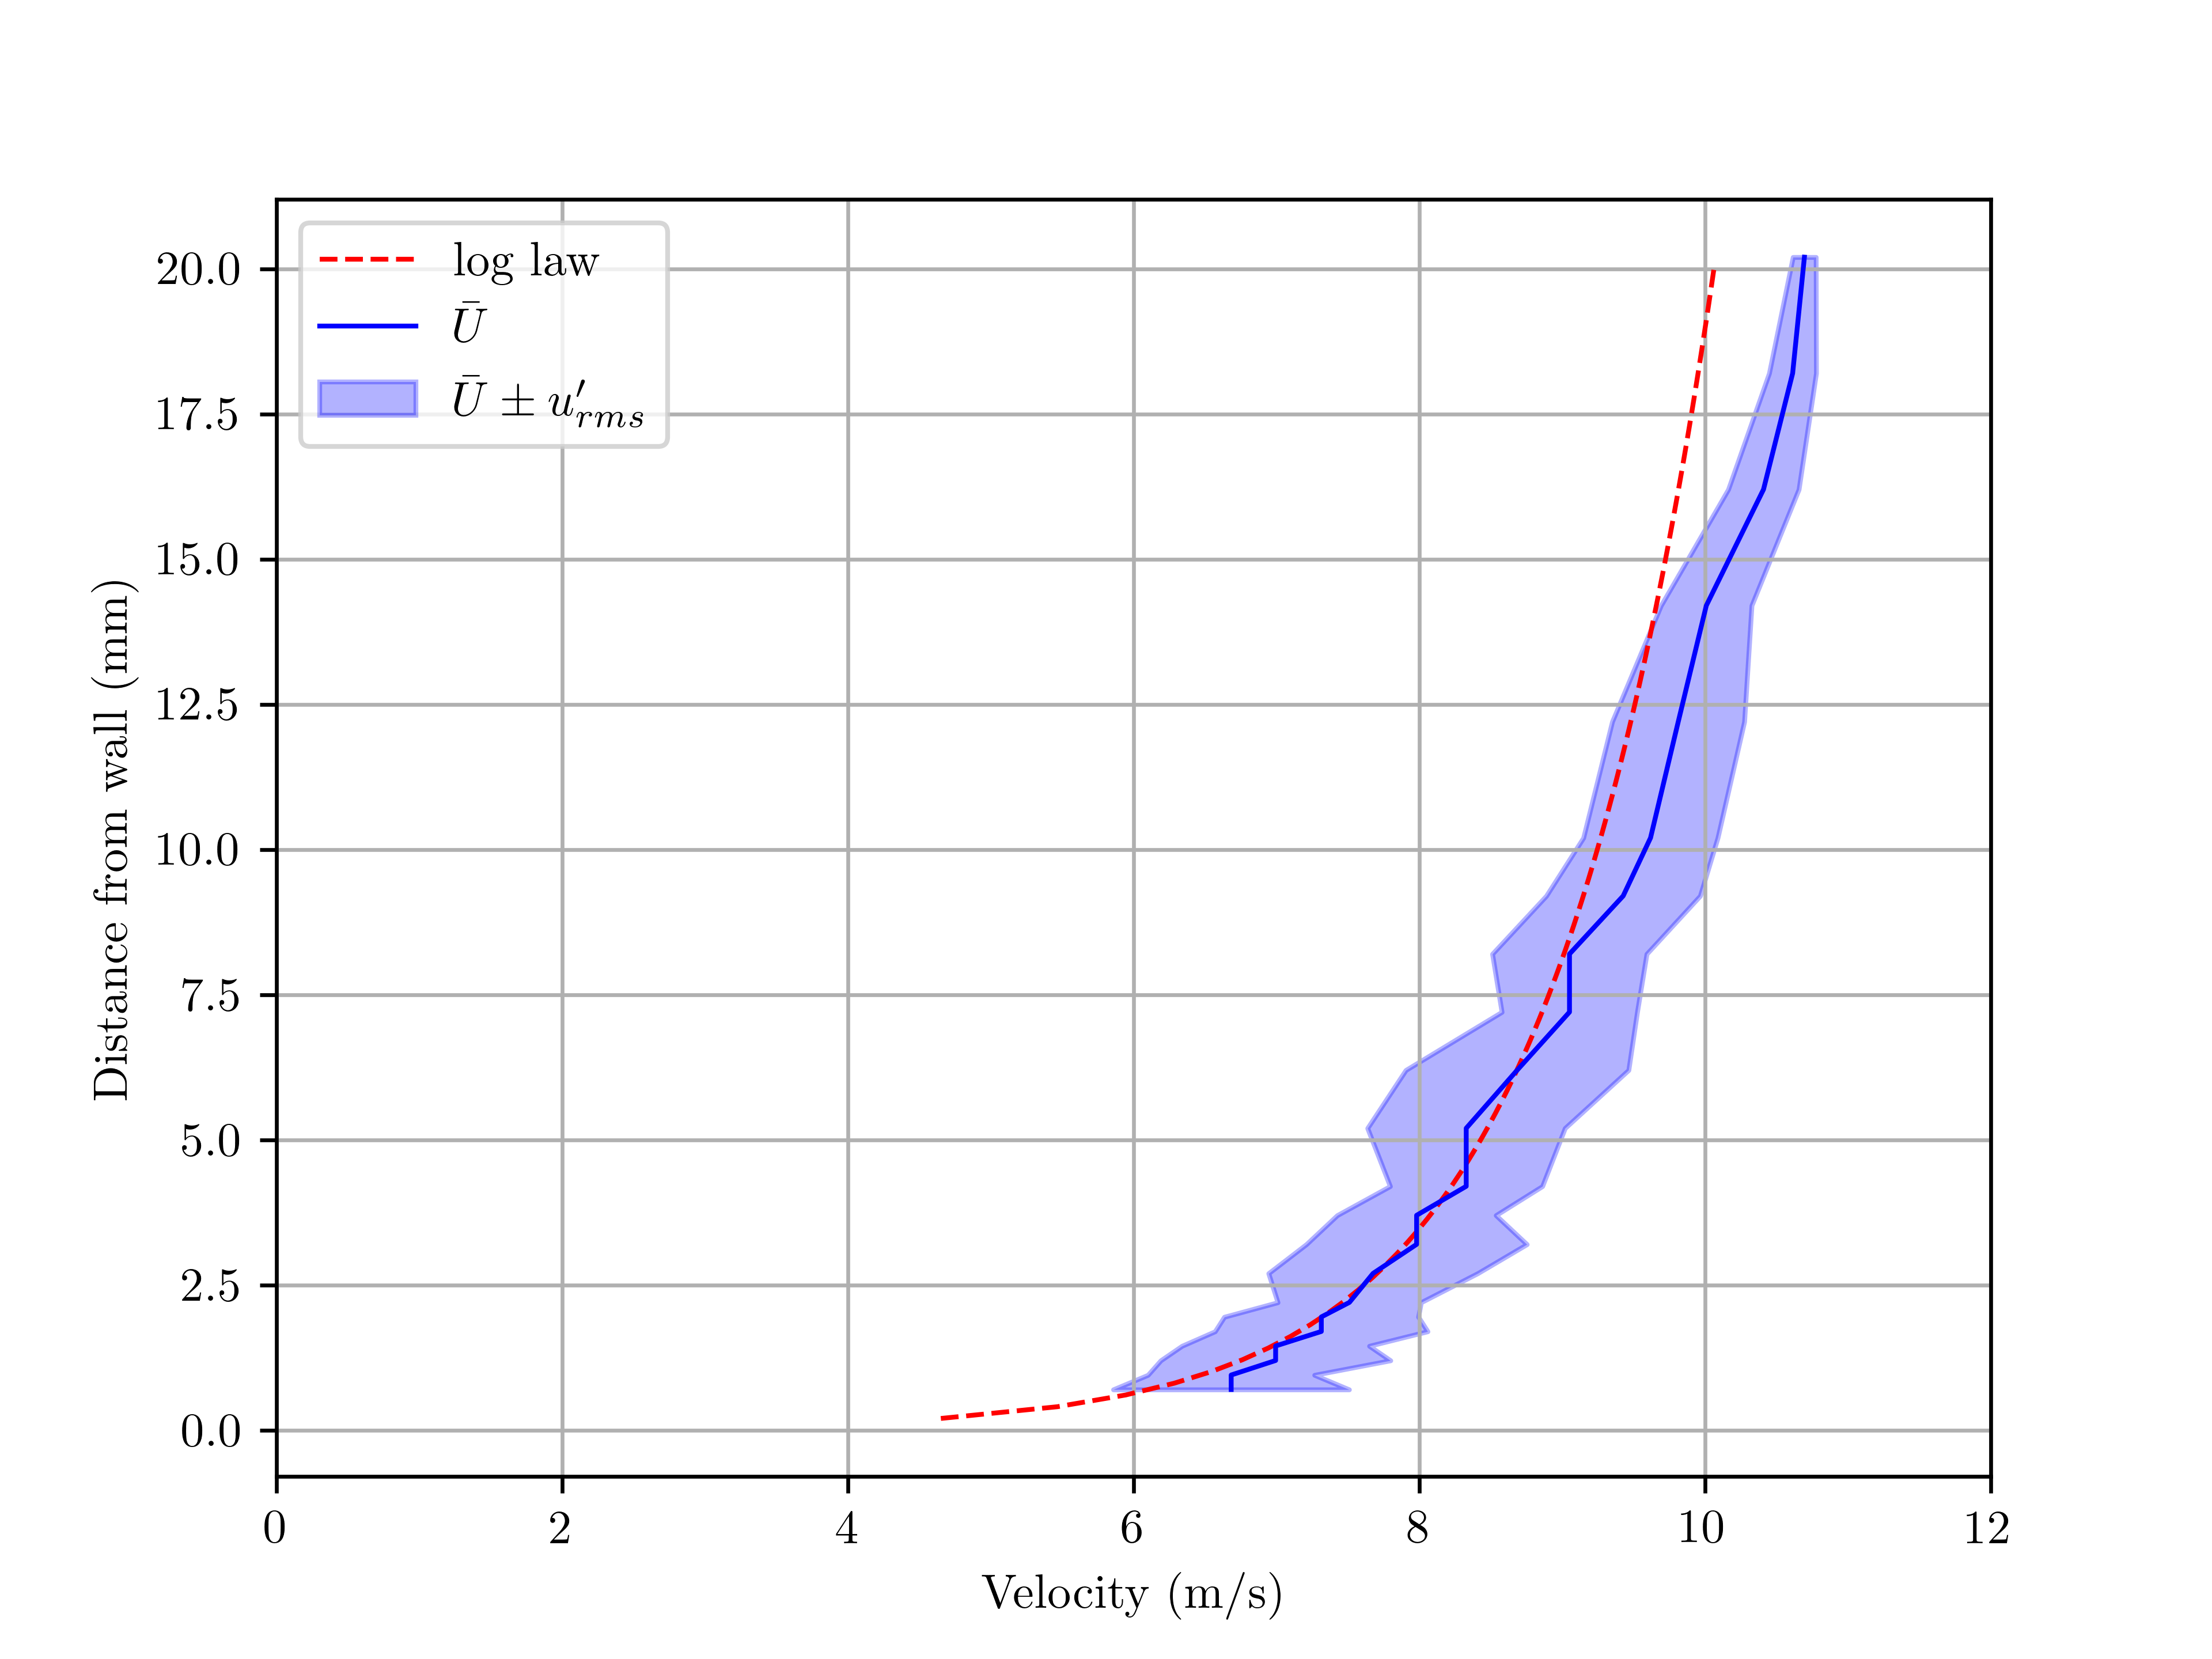
\includegraphics[width=0.99\textwidth]{turbulent_profile.png}
    \caption{Profile of turbulent boundary layer for a dial setting of 500}
    \label{fig:turbulent_profile}
\end{figure}

\begin{figure}[H]
    \centering
    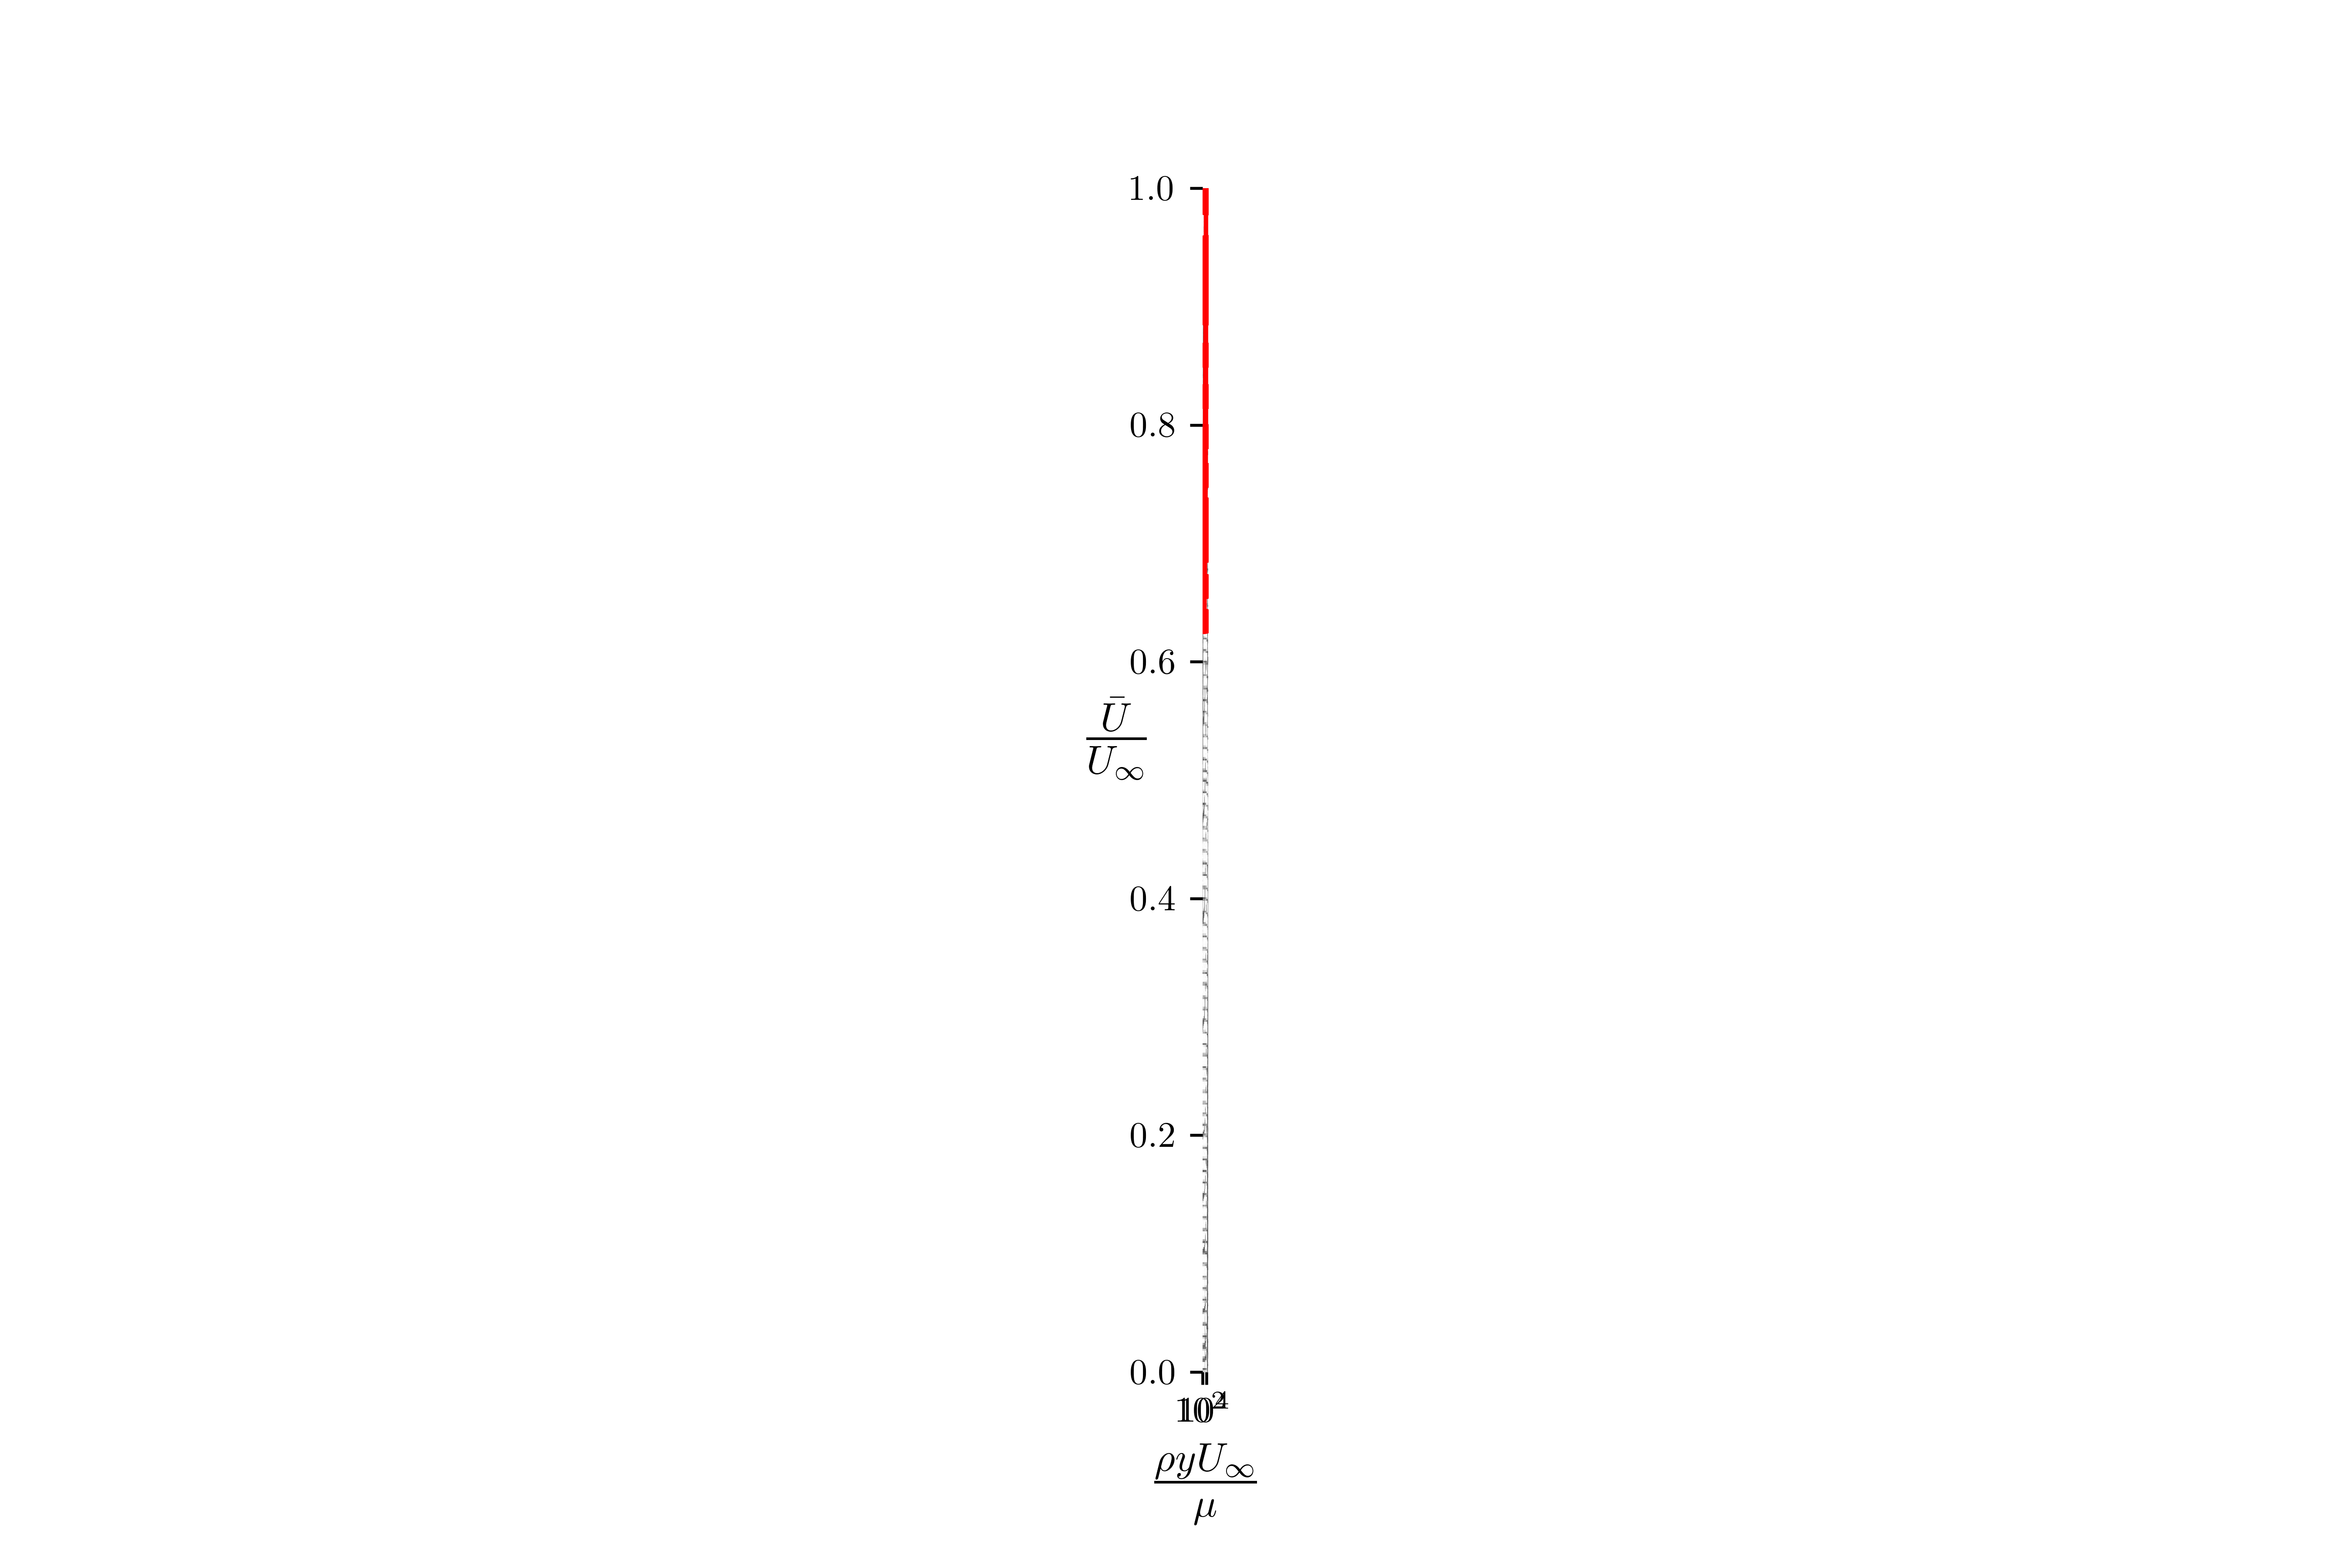
\includegraphics[width=0.99\textwidth]{clauser_data.png}
    \caption{Clauser plot of turbulent boundary layer profile for a dial setting of 500 \cite{handout}}
    \label{fig:clauser}
\end{figure}

\begin{figure}[H]
    \centering
    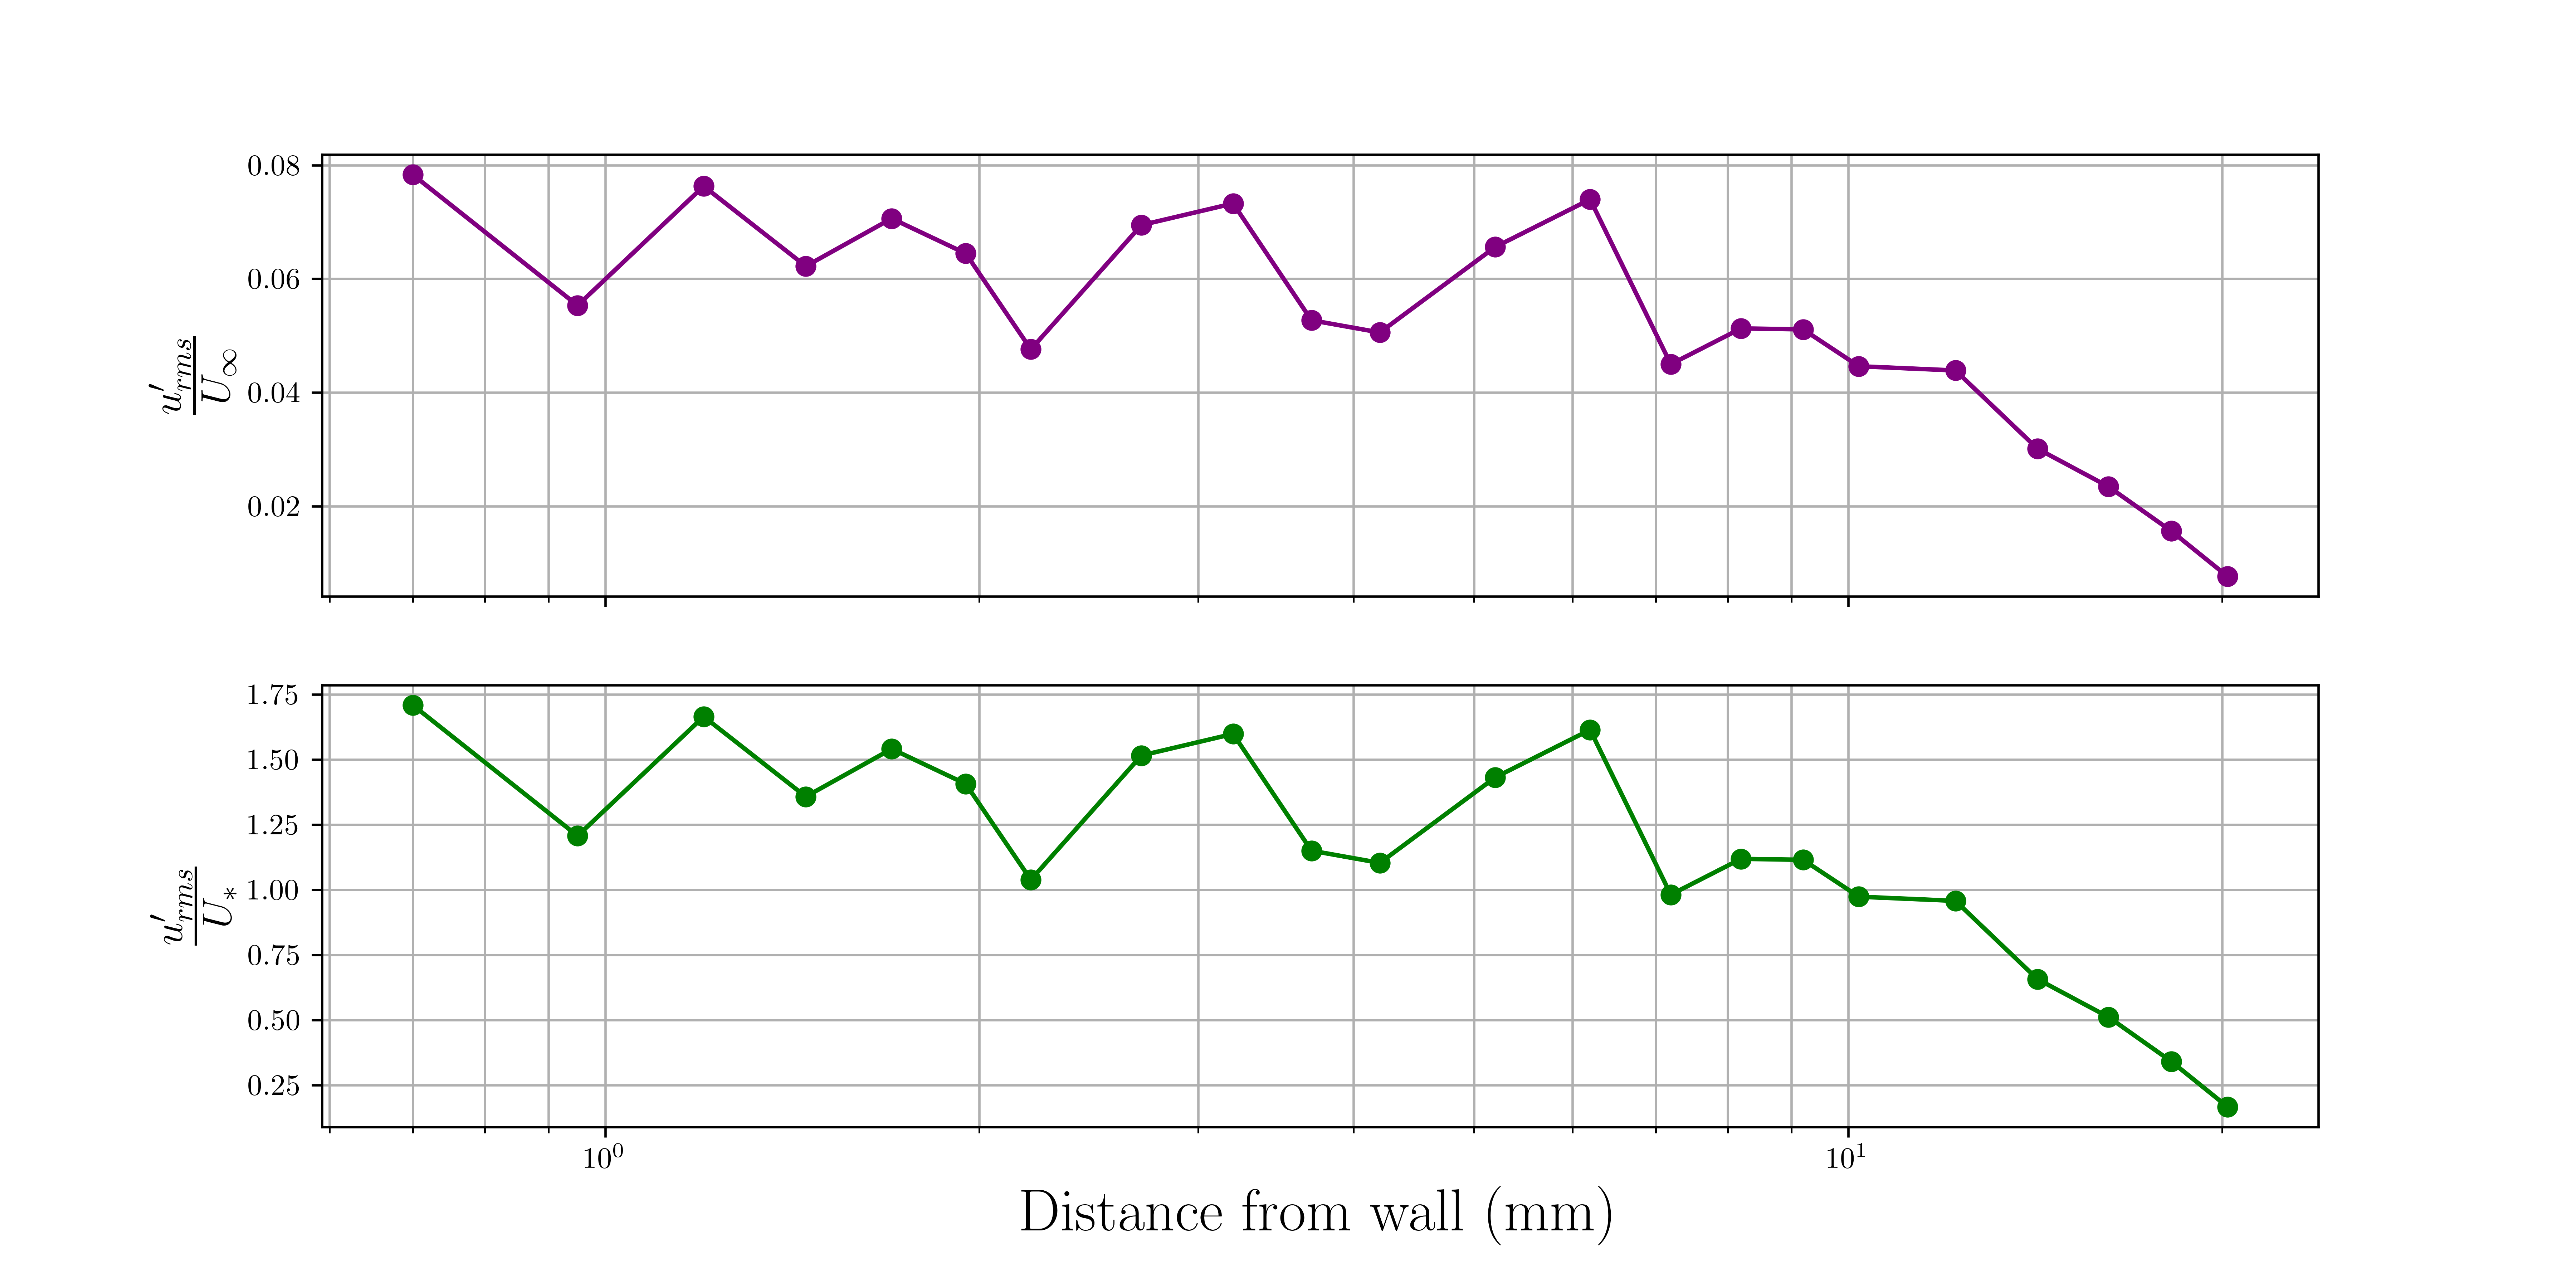
\includegraphics[width=0.99\textwidth]{u_fluctuation.png}
    \caption{Fluctuation of velocity with distance from the wall}
    \label{fig:fluctuation}
\end{figure}

%%%%%%%%%%%%%%%%%%%%%%%

\section{Discussion}
% Analyze and interpret the results, discussing their significance and any observations or trends.
%  laminar skin friction drag is smaller than turbulent skin friction drag, for the same inflow. 


% 2. Discuss the observations you have made.

%%% Kings law agrees with data?
Figure \ref{fig:calibration} shows the calibration curve for the hot wire anemometer.
The values for A and B were found as $A	= 1.589867$ and $B	= 0.596894$.
The data points obtained agree with the model of King's Law, with a mean squared error of $9.64\times 10^{-5}$.

%%% observations of turbulent regions in the boundary layer table 1 and figure 2
%%%

Figure \ref{fig:oscilloscope} shows the oscilloscope readings for the anemometer at various tunnel speeds.
Figure \ref{fig:oscilloscope_laminar} shows a fully laminar boundary layer as the voltage is smooth, 
however upon increasing tunnel speed increased fluctuations in voltage were observed, as seen in figure \ref{fig:oscilloscope_turbulent}.
From equation \ref{eq:small_kings}, this corresponds to fluctuations in velocity, which is an indication of turbulent eddies in the boundary layer.
Table \ref{tab:observations} shows the Reynolds number for the corresponding tunnel speeds.
From this the critical Reynolds number for each arangement lies between the observed laminar and transitioning row entries.
From lecture notes the critical Reynolds number for a flat plate is $Re_{xcr} \approx 5 \times 10^5$ \cite{notes} which agrees with the range $4-12 \times 10^5$.
For the protrusion, $Re_{xcr}$ was found to be in the range $4-70 \times 10^5$.
Only one Reynolds number was tested for the trip wire, and it was found to be turbulent so the value of $Re_{xcr}$ must be below $2.4\times 10^5$.
Further testing would be required to find more precise values of $Re_{xcr}$ for each arangement.

%%% Stethoscope observations for the different arangements
The stethoscope was used to measure the angle of the turbulent wedge formed downstream of the protrusion at a dial speed of 400.
This was done by slowly moving the stethoscope into the turbulent region until sufficient turbulent noise was heard at two points along the wedge.
The distance of the stethoscope from the wedge was then recorded, and the angle was calculated to be $\beta \approx 6^\circ$, as shown in figure \ref{fig:turbulent_wedge}.
It was also observed that the amplitude of noise varied over small distances from the measurement, which suggests that the edges of the turbulent wedge
are not well defined.

%%% Profile of the boundary layer

Figure \ref{fig:turbulent_profile} shows the profile of the boundary layer for a dial setting of 500.
Also shown is the log law approximation for the turbulent boundary layer of friction coefficient $C_f = 0.0042$.
These profiles match closely up to a distance of about 9mm from the wall, after which the velocity is larger than expected by the log law.
This is likely due to the boundary layer not being fully developed, as the flow is in the transition region at Aenometer.

% 3. How long are the intermittent patches of turbulence (spots) in the transition zone?
% calcualted from the local velocity and time difference between the spots

Table \ref{tab:spot_sizes} shows the size of turbulent spots and eddies for various setups and tunnel speeds.
The size of the turbulent spots for the flat plate were observed to increase from 35.4mm to 1580.4mm as the Reynolds number increased past $Re_{xcr}$.
The frequency of the spots was also observed to increase with Reynolds number.
This was expected as more turbulent spots are formed as the boundary layer transitions to turbulent flow.
These turbulent spots can coalesce to form larger spots as the boundary layer transitions to fully turbulent.
Turbulent spots were also observed for the protrusion which were found to be a similar size to the flat plate but at a higher Reynolds number.

% 4. Try to estimate the size of a typical eddy in the turbulent flow.
%% Done by measuring the time between the peaks of the velocity fluctuations and using local fluctuations in velocity

Table \ref{tab:spot_sizes} also shows the estimated sizes of typical eddies for various tunnel arangements and flow conditions.
Considering that the distance to the boundary layer is 0.2mm, the typical eddy size of ~5mm suggests that the actual eddies are much smaller than this.
However, these values are still applied as an indication of the size of the eddies.
For the flat plate case, disregarding the outlier, the typical eddy size decreased as the boundary layer transitioned further into turbulance.
This may be because more mixing of momentum has occured, and so the size of the typical eddies becomes smaller.
The protrusion case had similar sized eddies to the flat plate case.
However, the trip wire case had much larger eddies.

% 5. For the boundary layer profile, calculate the velocity ratio u'/U1
% where u'(y) is the velocity at height y and U1 ( is the free-stream velocity, and plot versus y, the distance
% from the surface. The points should also be plotted on the Clauser plot supplied. The
% demonstrator will provide you with the zero offset when the probe stop is just in
% contact with the plate (≈ 0.2mm).

The boundary layer profile is shown on the Clauser plot in Figure \ref{fig:clauser}.
The profile does not fit a constant friction coefficient line seen in the Clauser plot for the regions close to the wall and far from the wall.
For flow far from the wall the turbulent boundary layer is not fully developed and so does not agree with the clauser plot for a fully developed turbulent boundary layer.
The reason why the profile close to the wall does not fit is not known.

From interpolating the between linear regions on the Clauser the skin friction coefficient is estimated to be $C_f = 0.0042$.
The friction velocity is then calculated using \ref{eq:friction_velocity} as $u_* = 0.22$.
This was then used to plot figure \ref{fig:fluctuation}.

% 7. Calculate and plot versus distance from the wall on separate axes and discuss

Figure \ref{fig:fluctuation} shows the RMS velocity fluctuation with distance from the wall.
The velocity fluctuation decreases after about 6mm from the wall.
This is due to flow far from the wall taking longer to transition to turbulence.

\newpage

\section{Conclusion}
% Summarize the main findings of the experiment and draw conclusions based on the results.

A hot wire anemometer was calibrated and used to observe flow transition to turbulence over a flat plate, a protrusion, and a trip wire.
Flow at multiple Reynolds numbers was tested for each case and for the flat plate, $Re_xcr$ was found to agree with values common in literature.
Anemometer voltage recorded on an oscilloscope was used to observe and measure turbulent spots and eddies in the boundary layer at each Reynolds number.
The size and frequency of turbulent spots were observed to increase with increasing Reynolds number, and the size of typical eddies was observed to decrease.
The stethoscope was used to measure the angle of the turbulent wedge formed downstream of the protrusion by listening for turbulence.
The profile of the turbulent boundary layer was measured and used to estimate the skin friction coefficient on a Clauser plot.
A log law profile was found to fit the boundary layer closely for distance up to 9mm from the wall, and
$u'_{rms}$ was found to decrease after about 6mm from the wall.
The profile was observed to not fit the Clauser plot for regions close to the wall and far from the wall which was again thought to be due
to the Clauser plot being for a fully developed turbulent boundary layer.


%%%%%%%%%%%%%%%%%%%%%%%

\section{Appendix}

\begin{thebibliography}{9}
    \bibitem{handout}
    Cambridge University Engineering Department, \textit{Module 3A1: Transition to Turbulence Lab Handout}

    \bibitem{textbook}
    Frank M. White. \textit{Fluid Mechanics}. McGraw-Hill Education, 2004.

    \bibitem{notes}
    Li Jie, \textit{3A1: Boundary Layers Handout}. Cambridge University Engineering Department, 2023.
\end{thebibliography}

\end{document}


%% Honestly I have no clue why the clauser plot does not fit at the start.
%% I can believe that the boundary layer is not a fully developed as turbulent as the anemometer
